% THIS IS AN EXAMPLE DOCUMENT FOR VLDB 2012
% based on ACM SIGPROC-SP.TEX VERSION 2.7
% Modified by  Gerald Weber <gerald@cs.auckland.ac.nz>
% Removed the requirement to include *bbl file in here. (AhmetSacan, Sep2012)
% Fixed the equation on page 3 to prevent line overflow. (AhmetSacan, Sep2012)
%
\def\sharedaffiliation{%
\end{tabular}
\begin{tabular}{c}}
%
\documentclass{vldb12}
%\usepackage{anysize}
%\usepackage{geometry}
%\geometry{top=1in, left=1in, right=1in, bottom=1in,footskip=.25in}
%\marginsize{1in}{0.8in}{1in}{1in}%tblr
%\usepackage[showframe,bottom=0.2in,footskip=.25in]{geometry}
%\usepackage[left=1in, right=1in, top=1in]{geometry}
%\newcommand{\cmt}[2]{\textcolor{dkmag}{[#1: #2]}}
%\newcommand{\personname}[1]{\cmt{Personname}{#1}}
%\newcommand{\standout}[1]{\textit{\textcolor{dkmag}{#1}}}
\usepackage{graphicx}
%\usepackage[draft]{hyperref}
\usepackage{epstopdf}
\usepackage{hyperref}
\usepackage{url}
%\usepackage{relsize}
\usepackage{caption}
\usepackage{alltt}
%\usepackage{multicol}
%\usepackage{lineno}
\usepackage{subcaption}
%\usepackage{subfloat}
%\usepackage{float}
\captionsetup[subfigure]{labelformat=brace}
%\usepackage{classicthesis}
%\usepackage[a4paper,bindingoffset=0.2in,left=1in,right=1in,top=1in,bottom=1in,footskip=.25in]{geometry}
%\usepackage[left=1in,right=1in,top=1in,bottom=0.5in,footskip=.25in]{geometry}
\usepackage{algpseudocode}
%\usepackage[bottom=0.8in]{geometry}
%\usepackage{lipsum}
\usepackage{amsmath,amssymb}
%\usepackage{color, MnSymbol} %, hyperref} %wrapfig,
%\usepackage{balance, multirow, framed, caption, subcaption}  % for  \balance command ON LAST PAGE
\usepackage{algorithm}
\usepackage{algpseudocode}
%\usepackage{array,multirow,graphicx,tabularx}
%\usepackage{aliascnt}
%\usepackage{relsize}
%\usepackage{titling}
%\usepackage{fullpage} %,enumitem}
%\usepackage[T1]{fontenc}
%\usepackage{enumitem}
%\usepackage[shortlabels]{enumitem}
%\setlist{nolistsep}
%\setlist[enumerate]{nosep}

%
%\usepackage{fancyhdr}
%\usepackage{fullpage} %, hyperref}
%\usepackage{amssymb, amsmath, enumitem, titling, hyperref}
%\usepackage[standard]{ntheorem}
%%\usepackage[sort&compress]{natbib}
%\usepackage[top=0.65in, bottom=1.2in, left=0.95in, right=0.95in]{geometry}
% %\ifthenelse{\value{page}=1}
%          %{\setlength\headheight{40pt}}
%          %{\setlength\headheight{0pt}}
%					
%\usepackage[backend=bibtex,sorting=anyt, maxnames=7, firstinits=true]{biblatex} %hyperref=true,
%\renewcommand*{\bibfont}{\footnotesize}
%\bibliography{bib_rs}
%%\renewcommand{\baselinestretch}{0.9}
\def\sharedaffiliation{%
\end{tabular}
\begin{tabular}{c}}

\newcommand{\bigCI}{\mathrel{\text{\scalebox{1.07}{$\perp\mkern-10mu\perp$}}}}
\newcommand{\nbigCI}{\cancel{\mathrel{\text{\scalebox{1.07}{$\perp\mkern-10mu\perp$}}}}}
\newcommand{\rred}[1]{\textcolor{red}{#1}}
\newcommand{\mc}[1]{\mathcal{#1}}
\newcommand{\ignore}[1]{}
\newcommand{\comlb}[1]{{\vspace{2mm}\noindent \rred{\bf COMM(Dan):}}~ #1 \hfill {\bf    END.}\\}
\newcommand{\combabak}[1]{{\vspace{4mm}\noindent \bf  COMM(Babak):}~ {\em \rred{#1}}\hfill {\bf END.}\\}


\newcommand{\reva}[1]{{{{#1}}}}
\newcommand{\revb}[1]{{{{#1}}}}
\newcommand{\revc}[1]{{{{#1}}}}

\newcommand{\jout}{\mathbf{Y}}
\newcommand{\indep}{\textsc{Indep}}
\newcommand{\dans}[1]{{{\color{magenta} Dan Suciu: [{#1}]}}}
\newcommand{\babak}[1]{{\texttt{\color{blue} Babak: [{#1}]}}}
\newcommand{\danp}[1]{{\texttt{\color{red} Dan port: [{#1}]}}}
\newcommand{\corey}[1]{{\texttt{\color{blue} corey: [{#1}]}}}
\newcommand{\red}[1]{{\textbf {{\color{red} [{#1}]}}}}
\newcommand{\scream}[1]{{\texttt{\color{red}{\textbf{[{#1}]}}}}}


\newcommand{\att}{{\tau_{ATT}}}
\newcommand{\ate}{{\tau_{ATE}}}
\newcommand{\sch}{{\mathcal{S}}}
\newcommand{\rel}{{{R}}}
\newcommand{\sche}{{\mathcal{S}^e}}
\newcommand{\rele}{{{R}^e}}
\newcommand{\relei}{{{R}^e_{T_i}}}
\newcommand{\relt}{{{R}^e_{\trep}}}
\newcommand{\relti}{{{R}^e_{\trepi}}}
%\newcommand{\rel}{{{\textbf{R}}}}
\newcommand{\hm}{{\mathcal{S}}}
\newcommand{\crele}{{{R}^c}}
\newcommand{\echm}{{\mathcal{S}^{ce}}}
\newcommand{\cem}{{\textsc{Cem}}}
\newcommand{\mcem}{{\textsc{mCem}_{T_i}}}
\newcommand{\nnmwr}{{\textsc{Nnmwr}}}
\newcommand{\nnmnr}{{\textsc{Nnmnr}}}
\newcommand{\sbc}{{\textsc{SubC}}}
\newcommand{\prp}{{{P}_{\trep}}}
\newcommand{\prpi}{{{P}_{T_i}}}
\newcommand{\cv}{{{X}}}
\newcommand{\ccv}{{{\mc{X}}}}
\newcommand{\ccvi}{{{{cx}}}}
\newcommand{\cvi}{{{X_i}}}
\newcommand{\E}{\mathbb{E}}
\newcommand{\GSQL}{{{\textrm{ZaliQL}}}}
\newcommand{\delay}{\textsc{FlightDelay}}
\newcommand{\tre}{{{\mc{T}}}}
\newcommand{\trep}{S}
\newcommand{\trepi}{{{T}_i}}
\newcommand{\cvj}{{{X}_j}}
\newcommand{\cvij}{{{{X}}}}
\newcommand{\ccvj}{{\mc{X}}}
\newcommand{\ccvin}{{{\mc{X}'}}}
\newcommand{\ccvu}{{{\mc{X}}}}
\newcommand{\sub}{\bar{s}}
\newcommand{\LOGSPACE}{{\scriptsize $  \mathrm{LOGSPACE}$}}
\newcommand{\NLOGSPACE}{{\scriptsize $  \mathrm{NLOGSPACE}$}}
\newcommand{\PTIME}{{\scriptsize $  \mathrm{PTIME}$ }}

\newcommand{\ourproject}{{\textsc{Hume}}}
\newcommand{\ourlang}{{\textsc{HumeL}}}

\newcommand{\uiuc}{{UIUC}}
\newcommand{\cmu}{{CMU}}
\newcommand{\RP}{\emph{Robert Pennington}}
\newcommand{\TD}{\emph{Thomas Dunning}}

\newcommand{\ea}{\texttt{\bf E$_1$}}
\newcommand{\eb}{\texttt{\bf E$_2$}}
\newcommand{\ec}{\texttt{\bf E$_3$}}
\newcommand{\ed}{\texttt{\bf E$_4$}}
\newcommand{\ee}{\texttt{\bf E$_5$}}
\newcommand{\ef}{\texttt{\bf E$_6$}}

\newcommand{\Expl}{\texttt{Expl}}

\newcommand{\explq}{{explanation-query}}

\newcommand{\naivea}{\texttt{Alt-1}}
\newcommand{\naiveb}{\texttt{Alt-2}}
\newcommand{\incre}{\texttt{Incremental}}
\newcommand{\incrediff}{\texttt{Incremental-Diff}}

\newcommand{\tr}{1} %{\mathtt{t}}
\newcommand{\cn}{0} %{\mathtt{c}}




\newcommand{\A}{\texttt{A}}
\newcommand{\K}{\texttt{K}}
\newcommand{\deletelater}[1]{{\textbf {{\color{green} [{#1}]}}}}
\newcommand{\intervrel}{\texttt{intervened-relation}}
\newcommand{\attr}{\texttt{attr}}
\newcommand{\annot}{\texttt{annot}}
\newcommand{\supp}{\texttt{supp}}
\newcommand{\dom}{{\mathbb{D}}}
%\newcommand{\interv}{{\Gamma}}
\newcommand{\real}{{\mathbb{R}}}
\newcommand{\nat}{{\mathbb{N}}}
\newcommand{\explattr}{{\{E\}}}
%\newcommand{\change}{{\Delta}}
\newcommand{\bool}{{\textit{b}}}

\newcommand{\AP}{\texttt{AP}}
\newcommand{\highval}{\texttt{high}}
\newcommand{\midval}{\texttt{mid}}
\newcommand{\lowval}{\texttt{low}}
\newcommand{\aplow}{\texttt{poor}}
\newcommand{\aphigh}{\texttt{good}}
\newcommand{\dbnull}{\texttt{null}}
\newcommand{\relset}{\mathcal{R}}
\newcommand{\reltop}{{\mathcal{R}}_{top}}
\newcommand{\relbot}{{\mathcal{R}}_{bot}}
\newcommand{\attrset}{\mathcal{A}}
\newcommand{\attrtop}[1]{{\mathcal{A}}_{{top}, {#1}}}
\newcommand{\attrbot}{{\mathcal{A}}_{bot}}
%\newcommand{\featureset}{\mathcal{B}}
\newcommand{\db}{{D}}
\newcommand{\dbdom}{\mathbf{DB}}
\newcommand{\intervadditive}{{intervention-additive}}
\newcommand{\val}{{v}}
\newcommand{\valorig}{{u}}
%\newcommand{\dbdom}{\mathcal{D}}
\newcommand{\inputclass}{\mathcal{C}}
\newcommand{\intervene}{\mathcal{I}}
\newcommand{\tbaff}{{\tt{T_{Aff}}}}
\newcommand{\attaff}{{\tt{A_{Aff}}}}
\newcommand{\univ}{{{U}}}
\newcommand{\pk}{{\mathtt{pk}}}
\newcommand{\fk}{{\mathtt{fk}}}
\newcommand{\expl}{{\phi}}
%\newcommand{\pk}{{\tt \mathtt{\pk}}}
\newcommand{\sign}{{\tt \mathtt{sign}}}
%\newcommand{\expldom}{{\Phi}}
\newcommand{\select}{\tt {\textsc{Select}}}
\newcommand{\where}{{\tt \textsc{Where}}}
\newcommand{\with}{{\tt \textsc{With}}}
\newcommand{\distinct}{{\tt \textsc{distinct}}}
\newcommand{\groupby}{{\tt \textsc{Group By}}}
\newcommand{\from}{{\tt \textsc{From}}}
\newcommand{\ct}{{\tt \textsc{Count}}}
\newcommand{\create}{{\tt \textsc{Create}}}
\newcommand{\explanation}{{\tt \textsc{Explanation}}}
%\newcommand{\Pr}{{\tt {Pr}}}
\newcommand{\on}{{\tt \textsc{On}}}
\newcommand{\sqlwith}{{\tt \textsc{With}}}
\newcommand{\as}{{\tt \textsc{as}}}
\newcommand{\cascade}{{\tt \textsc{Cascade}}}
\newcommand{\sqland}{{\tt \textsc{And}}}
\newcommand{\sqlin}{{\tt \textsc{In}}}
\newcommand{\true}{{\tt true}}
\newcommand{\false}{{\tt false}}
\newcommand{\inmath}[1]{{\mathtt {#1}}}

\newcommand{\backwd}{\mathcal{B}}

\newcounter{enumQues}



\newcommand{\proj}[1]{{\Pi}}
\newcommand{\sel}[1]{{\sigma}}

\newcommand{\cut}[1]{}
\newcommand{\eat}[1]{}

%\newcommand{\tup}[1]{{\mathbf #1}}
\newcommand{\ul}[1]{{\underline{#1}}}
\newcommand{\commentresolved}[1]{}

\newenvironment{packed_item}{
\begin{itemize}
   \setlength{\itemsep}{1pt}
   \setlength{\parskip}{0pt}
   \setlength{\parsep}{0pt}
}
{\end{itemize}}

\newenvironment{packed_enum}{
\begin{enumerate}
   \setlength{\itemsep}{1pt}

  \setlength{\parskip}{0pt}
   \setlength{\parsep}{0pt}
}
{\end{enumerate}}

\newenvironment{packed_grep}{
\begin{description}
   \setlength{\itemsep}{1pt}
   \setlength{\parskip}{0pt}
   \setlength{\parsep}{0pt}
}
{\end{description}}

\newcommand{\ie}{{\em i.e.}} %\xspace}
\newcommand{\eg}{{\em e.g.}} %\xspace}
\newcommand{\etal}{{et al.}} %\xspace}
\newcommand{\aka}{{\em a.k.a.}\xspace}

\newcommand{\smalltt}{\tt \small}
\newcommand{\tinytt}{\tt \scriptsize}

\newcommand{\introparagraph}[1]{\textbf{#1.}}        % define own new subsection type: noindent, bold (textsc)

\newcommand{\angb}[1]{ {\langle {#1} \rangle}}                    % Set (as in \set{1,2,3}).

\newcommand{\set}[1]{\{#1\}}                    % Set (as in \set{1,2,3}).
\newcommand{\setof}[2]{\{{#1}\mid{#2}\}}        % Set (as in \setof{x}{x>0}).
\newcommand{\dtr}[0]{\twoheadrightarrow}        %
\newcommand{\bQ}[0]{\mathbf{Q}}        %
\newcommand{\bR}[0]{\mathbf{R}}        %
\newcommand{\bC}[0]{\mathbf{C}}
\newcommand{\bV}[0]{\mathbf{V}}
\newcommand{\mS}[0]{\mathcal{S}}
\newcommand{\mC}[0]{\mathcal{C}}
\newcommand{\bID}[0]{\mathbf{ID}}
\newcommand{\GCHQ}[0]{\textsc{GChQ}}
\newcommand{\CHQ}[0]{\textsc{ChQ}}
%\newtheorem{example}{Example}
%\newtheorem{pro}{Proposition}
%\newtheorem{proof}{Proof}
%\newtheorem{definition}{Definition}
%\newtheorem{theorem}{Theorem}
%\newtheorem{proposition}{Proposition}
%\newtheorem{def}{Definition}
%\usepackage[algoruled, lined]{algorithm2e}
%\usepackage{aliascnt}  		% ``hyperref’s \autoref command does not work well with theorems that share a counter:
						% it’ll always think it’s a Lemma even if it’s a Remark that shares the Lemma counter.
						% Load this package to fix it. No further intervention needed.''
						% Source: http://absatzen.de/thmtools.html (Jan 2009)
						% better: http://www.tug.org/applications/hyperref/manual.html (Nov 2009)
						% needs also: thm-patch.sty, parseargs.sty, aliasctr.sty ???
						% see section below for usage


\usepackage{graphicx}
\usepackage{balance}  % for  \balance command ON LAST PAGE  (only there!)

\begin{document}

% ****************** TITLE ****************************************

\title{ZaliQL: Causal Inference from Observational Data at Scale}
\numberofauthors{1}
\author{
  \alignauthor Babak Salimi  \ \  \ \ \  Corey Cole\ \  \ \ \    Dan R. K. Ports \ \  \ \ \  Dan Suciu
%
  \sharedaffiliation
  \affaddr{Department of Computer Science \& Engineering} \\
  \affaddr{University of Washington} \\
  \affaddr{\{bsalimi, drkp, suciu\}@cs.washington.edu, coreylc@uw.edu  }
}
% Ther
% possible, but not really needed or used for PVLDB:
%\subtitle{[Extended Abstract]
%\titlenote{A full version of this paper is available as\textit{Author's Guide to Preparing ACM SIG Proceedings Using \LaTeX$2_\epsilon$\ and BibTeX} at \texttt{www.acm.org/eaddress.htm}}}

% ****************** AUTHORS **************************************

% You need the command \numberofauthors to handle the 'placement
% and alignment' of the authors beneath the title.
%
% For aesthetic reasons, we recommend 'three authors at a time'
% i.e. three 'name/affiliation blocks' be placed beneath the title.
%
% NOTE: You are NOT restricted in how many 'rows' of
% "name/affiliations" may appear. We just ask that you restrict
% the number of 'columns' to three.
%
% Because of the available 'opening page real-estate'
% we ask you to refrain from putting more than six authors
% (two rows with three columns) beneath the article title.
% More than six makes the first-page appear very cluttered indeed.
%
% Use the \alignauthor commands to handle the names
% and affiliations for an 'aesthetic maximum' of six authors.
% Add names, affiliations, addresses for
% the seventh etc. author(s) as the argument for the
% \additionalauthors command.
% These 'additional authors' will be output/set for you
% without further effort on your part as the last section in
% the body of your article BEFORE References or any Appendices.

%\numberofauthors{4} %  in this sample file, there are a *total*
% of EIGHT authors. SIX appear on the 'first-page' (for formatting
% reasons) and the remaining two appear in the \additionalauthors section.


% Three authors sharing the same affiliation.

% You can go ahead and credit any number of authors here,
% e.g. one 'row of three' or two rows (consisting of one row of three
% and a second row of one, two or three).
%
% The command \alignauthor (no curly braces needed) should
% precede each author name, affiliation/snail-mail address and
% e-mail address. Additionally, tag each line of
% affiliation/address with \affaddr, and tag the
% e-mail address with \email.
%
% 1st. author

\frenchspacing


\maketitle

\begin{abstract}
Causal inference from observational data is a subject of active research and development in statistics and computer science. Many statistical software packages have been developed for this purpose.
However, these toolkits do not scale to large datasets.
We propose and demonstrate \GSQL: a SQL-based framework for drawing causal inference from observational data.
\GSQL\ supports the state-of-the-art methods for causal inference and runs at scale within PostgreSQL database system. \ignore{
\ignore{In addition, \GSQL\ includes several optimization techniques that significantly speedup causal inference, in both online and offline settings.}
\GSQL\ is designed as an extension for PostgreSQL database system.}
In addition, we built a visual interface to wrap around \GSQL. In our demonstration, we will use this GUI to show a live investigation of the causal effect of different weather conditions on flight delays.
\end{abstract}




\section{Introduction}
%\dan{7 pages}
\label{sec:introduction}

%\dan{this part is mostly done, only minor edits needed}

% Big data is used today in a wide range of domains, such as natural
% sciences (physics CITE, astronomy CITE, genomics CITE, biology CITE),
% social science and in particular measurements of human activity
% (e.g. recommendation CITE, personalization CITE),
% education~\cite{clauset-2015}, marketing and economics CITE, and MORE
% HERE.  The most successful type of application of Big data is {\em
%   predictive}: the data available, the \emph{seen} data, is used to
% infer a model that can predict features and trends of data that is not
% available, the \emph{unseen} data.  This potential for predictive
% analysis has generated the huge interest we see today in Big data, and
% has, in some sense, democratized data, by stimulating a huge number of
% ``data enthusiasts'' to collect, explore, analyze, integrate, and
% visualize data.  The term Big data is often used today to refer not
% just to the traditional features like volume, variety, velocity, but
% also to its wide availability to a broad range of users.


% lg1 - original commentout below at end; take care as this can lead to confusion
\ignore{Most data driven decisions today are based on purely predictive
analytics, which only finds associational dependencies and
correlations.  The danger is that naive data enthusiasts will
incorrectly interpret these predictive models as causal. While the distinction between causal and predictive analysis has
 been recognized, the conflation between the two is common which results in false discovery claims.}


To this day, {\em randomized experiments} (A/B testing) remain the gold standard for causal inference.
However, in many domains, controlled experiments are not feasible for ethical, economical or practical reasons \cite{rosenbaum2002observational}.
Statistical methods for causal inference can be used to draw conclusions from {\em observational studies}, i.e., without controlled experiments  \cite{rosenbaum2002observational,Rubin2005\ignore{,PearlBook2000,Spirtes:book01}}. Computational, physical, and social scientists all increasingly want to perform causal inference on big data from observational studies:
%Big data is most commonly observational and highly relational (e.g,
social networks, biological networks, sensor networks and more.
Unfortunately, current software for processing observational data for causal inference does not scale. R, Stata, SAS, and SPSS have packages such as {\em MatchIt} and {\em CEM}~\cite{ho2005,iacus2009cem}, but they are designed for single-table data and are cumbersome with large datasets. For example, we found that running CEM on a dataset with 5M entries takes up to an hour using Stata, R or SAS.

 Additionally, causal analysis is part of a larger pipeline that includes data acquisition,  cleaning, and integration. For large datasets, these tasks are better handled by a relational database engine, which provides most of the functionality needed for these tasks, and also scales up to large datasets. %% \dans{the previous sentence is cumbersome.  what we want to say is that causal analysis is part of a larger pipeline that includes data acquisition, data cleaning, and data integration; for large datasets, these tasks are best handled by a relational database engine, which provides most of the functionality needed for these tasks, and also scales up to large datasets.}
\ignore{A rich ecosystem of tools and organizational requirements further encourage SQL database storage. Transferring
data from DBMS to statistical softwares or connecting these
softwares to DBMS can be error prone, difficult, time consuming and inefficient. For these
cases, it would be helpful to push statistical methods for causal inference into the DBMS.
\ignore{\corey{should go over the scalability / current tool problem here before jumping into the} solution?}}


In this demonstration, we propose \GSQL,\footnote{ The prefix Zali refers to
  al-Ghzali (1058-1111), a medieval Persian philosopher. It is known
  that David Hume (1711-1776), a Scottish philosopher, who gave the
  first explicit definition of causation in terms of counterfactuals,
  was heavily influenced by al-Ghzali's conception of causality.}
  a SQL-based framework for drawing causal inference within the DBMS. \GSQL\ takes the first step towards truly scalable causal inference by modeling it as a data management problem. We demonstrate that
  causal inference can be approached from this perspective, and that doing so is key to scalability and robustness.  \GSQL\ supports state-of-the-art methods for causal inference and runs at scale within a database engine.  \ignore{ The framework \ignore{is designed and implemented as an extension for PostgreSQL object-relational database
systems and} includes a series of optimization techniques that allow it to
scale to billions of records.}




\begin{figure}\center
 \includegraphics[scale=0.20]{Figures/System-Overview.png}
  \vspace{-3.3mm} \caption{ZaliQL architecture}

  \label{fig:arch}
  \vspace{-3mm}
\end{figure}


\begin{figure} \center
  \includegraphics[scale=0.21]{Figures/Matching-Flowchart.png}
  \vspace{-3mm}\caption{Causal analysis workflow}

\label{fig:flowchart}
\vspace{-0.3cm}
\end{figure}

\vspace{-.3cm}

\section{System Architecture}

The overall architecture of \GSQL\ is shown in Fig. \ref{fig:arch}.
% \dans{corey addressed - start by saying that data is stored in a Postgres system}
The API is a set of functions that support causal inference on data stored in a PostgreSQL DBMS. %\footnote{\url{http://postgresql.org/}}
The API will be packaged as a PostgreSQL extension. %and will be released in
%PostgreSQL Extension Network.\footnote{\url{http://pgxn.org/}}
The \GSQL\ API is modeled after the MatchIt and CEM toolkits
\cite{ho2005,iacus2009cem} and includes methods for drawing causal inference from relational data. For demonstration and exploration purposes, \GSQL\ also includes a web GUI
(see Fig. \ref{sfig:demo-tutorial}). %It can be configured with the user's databases URL after they have installed the \GSQL\ Postgres extension. The  GUI be hosted remotely on a server or locally on \ignore{
%The interface consists of three tabs : Setup, Matching Summary, and Analysis.
%}

\ignore{
\dans{We should add more details here: describe the main functions
  that the API supports; mention that they generate and optimize SQL
  queries.}}

\begin{figure*} \centering
\hspace*{-.1cm}
\includegraphics[scale=0.16]{Figures/Demo-Tutorial.png}
\caption{Demonstration screenshot described in Section \ref{sec:dd}}
\label{sfig:demo-tutorial}
\end{figure*}

\vspace{-.3cm}
\section{Demonstration Details}
\label{sec:dd}
Modern causal analysis is an iterative process, as  illustrated in Fig \ref{fig:flowchart}.
An analyst acquires and integrates data from multiple sources,
generates a hypothesis, pre-processes the data with a matching  method (explained below), and then finally
 conducts the causal analysis. Frequently, this process needs to be repeated with a new matching
  method, a new hypothesis or new datasets \cite{IacKinPor09}.
  We demonstrate this workflow in \GSQL\ through several causal investigations on integrated flight and weather datasets. \ignore{on two,
  large datasets that we downloaded from the Web and integrated in PostgreSQL.}

\ignore{
 In this demonstration, we will use \GSQL\ to quantify the causal effect of
 different weather conditions on flight departure delay. }

    {\bf Data:} The analysis will be conducted on a spatio-temporal join of the following two datasets:
(a) {\it Flight dataset (105M entries)}: collected by the US
Department of Transportation.\footnote{\url{http://www.transtats.bts.gov/}} It contains
records of more than 90\% of US domestic flights of major airlines
from 1988 to the present. It includes attributes such as FlightDate, OriginAirportID,
CarrierID, CRSDepTime (scheduled departure time), and DepDelay (departure delay).
(b) {\it Weather dataset (40M entries):} collected using the Weather Underground API.\footnote{\url{https://www.wunderground.com}}
It contains historical weather data for related to flights. It includes attributes such as Code (Airport ID),
Date, Time,  Visim (visibility in km),
  Tempm (Temperature in C$^{\circ}$)
  Wspdm (wind speed in kph), Pressurem (Pressure in mBar), Precipm  (Precipitation in mm), Snow (binary), Thunder (binary).






\ignore{
\begin{figure*}
\begin{subfigure}{0.50\linewidth}
\centering
\includegraphics[scale=0.13]{Figures/Setup.png}
\label{sfig:testc}
\end{subfigure}\hfill
\begin{subfigure}{0.47\linewidth}
\centering
\includegraphics[scale=0.13]{Figures/Matching-Summary.png}
\label{sfig:testd}
\end{subfigure}\hfill
\caption{Demonstration Screenshot described in Section \ref{sec:dd}}
\label{fig:eteresult}
\end{figure*}
}









 \ignore{
 The analysis will be conducted on
 {\em flight data (105M eateries)}-collected by the US Department of Transportation (U.S. DOT)- and  {\em weather dataset} (10M eateries)-gathered using the weather underground
API. }

 \ignore{
 The {\em flight dataset} we use was collected by the US Department of Transportation (U.S. DOT) \cite{flightdata}. It contains
records of more than 90\% of US domestic flights of major airlines
from 1988 to the present. The {\em weather dataset} was gathered using the weather underground
API \cite{Weatherdata}.  \ignore{Its attributes are also presented in Table
\ref{tab:attlist}. In addition, we pre-computed two other attributes
AiportTraffic and CarrierTraffic. The former is the total number of
flights occur in the origin airport of a flight one hour prior to the
flight departure time, the latter is the same quantity restricted to
the flights from the same carrier.  We managed to acquire and clean
35M weather observations between 2000 and 2015.} These datasets are
integrated by a spatio-temporal join.}



\ignore{

        \caption{Weather dataset}
    \end{subtable}
 \vspace{-0.1cm}   \caption{\bf{List of attributes from the flight(a) and weather(b)  datasets that are relevant to our analysis.}}
\label{tab:attlist}
\end{table}
}









\ignore{
\begin{example} \em \delay (cont.) \ \em   Suppose we want to explore the effect of the low-pressure (treatment) on flight departure delays (outcome).  The direct comparison of
delay between flights that happen during low-pressure (treated groups) and opposite (control group) is misleading.  It is known that high pressure is generally associated with clear weather,    while low-pressure is associated with unsettled weather, e.g.,
    cloudy, rainy, or snowy weather\ignore{\cite{weba2,barometricpressureheadache:article}}. Thus, as shown in Figure \ref{fig:cv}, factors such as thunder, snow, visibility confound pressure and delay. Therefore, conducting any sort of predictive analysis identifies
    low-pressure as a predictor for flight delays.
  However, low-pressure does not have any causal impact on departure delay
    (low-pressure only requires longer takeoff distance) \cite{FAA08}. In this demonstration, by conducting a careful causal analysis using \GSQL, we show that low-pressure is only a correlated attribute with flight delays and has no significant causal impact on flight delay.

    \ignore{By performing a careful casual analysis
    \GSQL\ found that other attributes such as thunder, low-visibility, high-wind-speed and
    snow have the largest causal effect on flight delays (see Sec. \ref{sec:endtoend});
  this is confirmed by the results reported by the FAA.}
\end{example}
}

 {\bf Data exploration:} Our demonstration starts by exploring the effect of different weather features
 on flight departure delay. As an example, we show that 11\% of flights were delayed
when pressure was low, but only 0.4\% of flights
when pressure was high. This suggests that pressure is {\em inversely correlated} with flight delay
(as pressure goes down, flights tend to be more delayed).
However, after grouping by variables like airport, airline, and other weather features,
flight delay frequency declined from 11\% to almost 0\%.\footnote{This phenomenon
is known as Simpson's paradox and arises frequently in observational studies \cite{pearl2014comment}.
We demonstrate that the issue could be avoided by conducting a careful causal analysis.
} In light of this, does low pressure really affect flight delays?



 {\bf Causal questions:} In this step, we define the following {\em causal questions}:
Q1: Does low air pressure cause flight departure delays?
Q2: Which weather features are major causes of departure delays?
Q3: Do the findings to the previous question differ between major airports in the states? We answer these questions using \GSQL\ by
 \vspace{-0.24cm}
\begin{itemize}
  \item specifying DepDelay as our outcome of interest (effect)
as shown in Fig. \ref{sfig:demo-tutorial}(a).
 \vspace{-0.33cm} \item specifying a set of binary treatments (causes)
 \newline
 that might affect DepDelay,
 as shown in Fig. \ref{sfig:demo-tutorial}(b).
In particular, the following binary treatments will be created:
LowVisibility (1 if Visim$<1$ ); \
%; 0 if Visim$>5$
  HeavySnow (1 if Precipm$>0.3$ and Snow$=1$); \
  HighWindSpeed (1 if Wspdm$>40$; 0 if Wspdm$<20$); \
  Thunder; \ LowPressure (1 if Pressurem$<1009.14$; 0 if Pressurem$>1022.69$).

   \item specifying a subset of data that is relevant to the analysis.  We select five US airports  with high rate of weather-related delay, namely,
    San Francisco (SFO), John F. Kennedy (JFK), Newark Liberty (EWR),
    \newline
    George Bush (IAH), and LaGuardia Airport (LGA).
\end{itemize}

\ignore{
(1) specifying DepDelay as our outcome of interest (potential effect)
as shown in Figure \ref{sfig:demo-tutorial}(a),
(2) specifying a set of binary treatments (potential causes) that might affect DepDelay,
 as shown in Figure \ref{sfig:demo-tutorial}(b),
In particular the following binary treatments will be created:
 LowVisibility (1 if Visim$<1$; 0 if Visim$>5$); \
  HeavySnow (1 iff Precipm$>0.3$ and Snow$=1$); \
  WindSpeed (1 if Wspdm$>40$; 0 if Wspdm$<20$); \
  Thunder; \ LowPressure (1 if Pressurem$<1009.14$; 0 if Pressurem$>1022.69$)     \ignore{
      As shown in Figure \ref{sfig:demo-tutorial}(b) Clicking on the {\it ADD TREATMENT}, {\it ADD COVARIATE}, and {\it ADD OUTCOME} buttons will trigger a dialog allowing
  further customization on the discretization and matching methods.
These dialogs will also allow the user to incorporate other columns (e.g. snow is defined as $iff Precipm> 0.3 and
Tempm< 0$) and input SQL for custom discretization methods.} and (3) specifying a subset of data that is relevant to the analysis.  We select five US airports  with high rate of weather-related delay, namely, San Francisco (SFO) , John F. Kennedy (JFK), Newark Liberty (EWR), George Bush (IAH), and LaGuardia Airport (LGA).
}


 { \bf Computing ATE}: In causal inference, the objective is usually to quantify
 the causal effect of a binary treatment on an outcome.
 A common measure of effect is {\em average treatment effect} (ATE).
 ATE is defined as the difference in expected values of the treated
 and untreated units.\footnote{In causality literature, subjects of a
   study --
  e.g., patients in a clinical trial -- are called units. In our case, each flight
   is considered a unit.}
   \ignore{\dans{this part is good.
    But I would make it a bit more tutorial-style.  Start by
    saying that in causal analysis we want to study
    the causal effect of a binary attribute called treatment, on an attribute
    alled outcome.  The ATE is defined as the difference in expected
    values of the treated and untreated units.
    (Add a footnote saying that records are called units in causal analysis).
     Then continue with what you have here, by referring to Q1 above:} }
     For example for Q1, \GSQL\ computes ATE as

     \vspace*{0.2cm}
{\small
   \centering  $ \ \ \E[ \text{DepDelay} | \text{LowPressure}=1] - \E[ \text{DepDelay} | \text{LowPressure}=0] $ }
    \vspace*{0.15cm}

\noindent where, $\E[ \text{DepDelay} | \text{LowPressure}=x ]$, $x=(0,1)$ is
  computed by taking the emetical average of  DepDelay where LowPressure is  $x$.
  It is a  common measure to compare an
  outcome (DepDelay) in the {\em treated group},  those subjects
  (flights) that receive a treatment (LowPressure=1), with the {\em control group} (LowPressure=0).
\ignore{\dans{For the next sentence, can you refer to Fig. 3.
  There the user has selected the treatment visibility (Visim)
   and the outcome is DepDelayMinutes.  (Acually, can you update
    the figure so that the treatment is LowPressure).  If we compute
    the ATE for LowPressure on DepDelay, the result is  (give concrete number).}}
    We show that for LowPressure, ATE is 10 minutes.
    This is relatively large and suggests pressure affects DepDelay.
    However, it is known that LowPressure alone does not actually cause departure delay.
    Where, then, is this difference coming from, and how do we account for it?


%%%%%%%%%%%%%%%%%%%%%%%%%%%%%%%%%%%%%%%%%%%%%%%%%%%%%%%%%%%%%%%%%%%%%%%%%%%%%%%%%%% check ba;ance


\ignore{
 \paragraph{\bf Confounding variables:} \dans{Use this as an excuse to continue the mini-tutorial.  The first 1-2 setnences should be general, saying that  causal analysis conditions on confounding variables. Then you immediately make it concrete and say that, if the confounding variable is LowVisibility, then the ATE for LowPressure on DepDelay decreases significantly.} We address this question, by demonstrating that the comparison of DepDelay between the treated and control groups is misleading due to the existence of the so-called {\em  confounding influence} of other variables such as visibility, snow and thunder.  In fact we show that, LowPressure is highly associated with unsettled weather conditions such as LowVisibility. For instance the average of LowVisibility in the treated group is much less than
  the opposite group. Thus, it is unclear that the observed DepDelay difference between the groups is causes by LowPressure or LowVisibility. This scenario, as shown graphically in Figure \ref{fig:cv}, demonstrates that in the presence of {\em confounding variable} (a.k.a, {\em covariates}) the treated and control groups are very different and comparing them without accounting for the confounding variables could be misleading.
}

\ignore{ \dans{Use this as an excuse to continue the mini-tutorial.  The first 1-2 sentences should be general, saying that  causal analysis conditions on confounding variables. Then you immediately make it concrete and say that, if the confounding variable
  is LowVisibility, then the ATE for LowPressure on DepDelay decreases significantly.}}
 {\bf Confounding variables:} The difference is a product of {\em confounding variables}
  that make it difficult to establish a causal link between a treatment and outcome.
  We will show that the observed positive effect of LowPressure
  was actually the result of the confounding influence of other factors such as low visibility, snow, and thunder.
     Specifically, we show that, LowPressure is highly associated with unsettled weather conditions
    such as LowVisibility (Fig. \ref{fig:cv}). For instance, the average of LowVisibility in the treated group is much less than
  the opposite group. Thus, it is unclear that the observed DepDelay difference between the groups is caused by LowPressure or LowVisibility.


\ignore{
  This scenario, as shown graphically in Figure \ref{fig:cv}, demonstrates that in the presence of {\em confounding variable} (a.k.a, {\em covariates}) the treated and control groups are very different and comparing them without accounting for the confounding variables could be misleading.
}
{
\begin{figure} \centering
\hspace*{.3cm}\includegraphics[scale=0.35]{figures/counf.png}
\caption{Confounding influence}

\label{fig:cv}
\vspace{-0.5cm}
\end{figure}}
 {\bf Adjusting for confounding variables:} {
In order to draw valid causal conclusions, we need to adjust for confounding influences.
Conceptually, adjusting for one confounding variable is easy.  First, we partition the data into groups with similar confounding influence measures.
 Then, we compute the ATE as the weighted average of the effects \emph{in each group}.
 However, real-world causal inference requires many confounding variables.
  For example, LowPressure has more than ten confounding variables
 (some of them are shown in Fig. \ref{fig:cv}).
 In such a case, the groups often become too specific, lacking enough units in each group to enable a meaningful estimation of the ATE.


 Sophisticated techniques are required to adjust for a large set of confounding variables. \GSQL
 implements two dominant approaches used in social science and statistics, namely,
  {\em coarsened exact matching (CEM)} and {\it propensity score matching (PSM)}
 \cite{IacKinPor09,Rubin1983b}.
 The goal of matching is to prune data so that
the remaining {\em matched} data have better \emph{balance}
between the treated and control groups. That is, the empirical
distributions of the confounding variables in the treated and control
groups are similar after matching.
Once the two groups are balanced, any observed difference of the
outcome between the two groups can be attributed to the treatment. In
our demo, (1)\ for each treatment, we select a set of covariates
deemed to confound the treatment and DepDelay (Figure \ref{sfig:demo-tutorial}(c)) and
  (2)\ we select a matching method and adjust its tuning parameters.



{\bf Checking Balance:}  In this step, we check whether the
matching process  successfully improved the covariates' balance. In particular,
 we compare the distribution for each covariate between the
 treated and control group on the matched data
 (this will be done for all treatments). For this task, \GSQL\  provides
 numerical and visual summaries such as mean difference and quantile-quantile plots:
  see Fig. \ref{sfig:demo-tutorial}(d,e). \ignore{
(2)  we can perform different matching methods using different
        parameters, showing that different methods trade off balance and size of matched data% to demonstrate the advantages and disadvantage of different methods.

      The main objective of this step is to demonstrate the typical workflow of
       causal inference from observational data.
        As shown in Figure \ref{fig:flowchart}, it
        consists of the iterative process of matching and balance checking. This highlights the demand for tools such as \GSQL\, which perform matching at scale.
}


     {\bf Answers to our causal questions:} %\dans{We should give here concrete answers to the queries Q1,Q2,Q3.  Then add a sentence saying that we will perform other causal analysis during the demo}
In this step,  we answer the causal questions created at the very first step of the demonstration using
\GSQL. For Q1, we show that LowPressure has no significant causal effect on DepDelay.
We show that other treatments \emph{do} have significant causal effect on departure delays (Q2), and further that these causes are different for different airports in the study (Q3, Figure \ref{sfig:demo-tutorial}(f)).
   \ignore{
       \item for each treatment we compute ATE on the associated balanced matched data
      \item we evaluate the statistical significance of the obtained
        result by performing statistical tests, such as the chi-square test.
          \item For Q3 we report the major causes of flight delay at the airports under study.}
For Q3, we report the major causes of flight delay at the airports under the study are
     actually different. We validate the statistical significance of our findings with t-tests, and show that the identified causes match
FAA reports. % \footnote{\url{https://www.faa.gov/}}
\ignore{For example, the runway configuration at SFO makes the airport
unusually susceptible to delays in low-visibility conditions~\cite{faa-sfo}.}
% which reported the following major weather-related
% causes:
% snows, thunders and wind at EWR; thunder and fog at IAH;
% snows and visibility at JFK; snows at LGA; visibility at SFO;





{\bf Scalability:} Finally, we demonstrate
  scalability by letting users interactively run queries on this large
   dataset--which would take the existing toolkits hours. As seen in Figure \ref{sfig:demo-tutorial}(g),
\GSQL\ can process 100M entries in less than a few minutes, whereas
existing systems like R, SPSS or SAS,
 take up to an hour to process just 5M entries. \footnote{We note that
   the
   developers of statistical software packages for CEM have identified
   \GSQL\ as a more scalable approach: see \url{http://gking.harvard.edu/cem}.}

%\vspace{-.2cm}
\section{Internals}
\subsection{Basic Formalism}

The basic causal model in statistics is called the
\ignore{Neyman-Rubin Causal Model (NRCM) (also referred to as}
{\em potential outcome framework} (POF) \cite{Rubin2005}.
In this model, we are given a table with $N$ rows called {\em units} indexed by $i=1 \ldots N$ (see
Table~ \ref{fig:causal:inference}).  The binary attribute $T$ denotes {\em treatment assignment}.
%sr: already in first para. ($T=1$ means the unit was treated; $T=0$ means the unit was subjected to control);
$X$ is a vector of
background characteristics, (e.g., airport, airline, weather \ldots) of each unit,
called {\em covariates}, unaffected by treatment; and the two
attributes $Y(0), Y(1)$ represent {\em potential outcomes}: $Y(1)$ is
the outcome of the unit if it is exposed to the treatment and $Y(0)$
is the outcome when it is exposed to the control.

%For any attribute $T$, we write $T_i$ for the value of the $i$'s unit.
The {\em treatment effect}
caused by the treatment $T_i$ for the $i$th unit  is defined as $Y_i(1)-Y_i(0)$.
The goal of causal analysis is to compute the {\em average treatment
  effect (ATE)}:   $$ATE = \E[Y(1)-Y(0)] = \E[Y(1)] - \E[Y(0)].$$


\begin{figure}
  \centering
{\scriptsize
  \scalebox{0.7}{\begin{tabular}{|c|c|c|c|c|c|} \hline
    Unit & Covariates & Treatment & Treatment & Control & Causal  Effect \\
   & $X$ & assignment $T$ & outcome $Y(1)$ & outcome $Y(0)$ & $Y(1)-Y(0)$ \\
    \hline
    1 & $X_1$ & $T_1$ & $Y_1(1)$ & $Y_1(0)$ & $Y_1(1) - Y_1(0)$ \\
    2 & $X_2$ & $T_2$ & $Y_2(1)$ & $Y_2(0)$ & $Y_2(1) - Y_2(0)$ \\
    $\ldots$ & $\ldots$ & $\ldots$ & $\ldots$ & $\ldots$ & $\ldots$ \\
    N & $X_N$ & $T_N$ & $Y_N(1)$ & $Y_N(0)$ & $Y_N(1) - Y_N(0)$ \\ \hline
  \end{tabular}}
}
\caption{The Potential Outcome Framework}
  \label{fig:causal:inference}
  \vspace{-3mm}
\end{figure}
\noindent
The so-called {\em fundamental problem of causal inference} %(FPCI)
is that
for each unit we only know either $Y(1)$ or $Y(0)$ but not both.
\ignore{\danp{Can we add an example to make this more intuitive,
 since it's important e.g.: each individual flight has either
    LowPressure=1 or =0, not both}} For example, each individual
flight has either LowPressure=1 or LowPressure=0, so only one of DepDelay(1)
or DepDelay(0) is available for each row.
Thus, further assumptions are needed for estimating ATE. \ignore{
\cite{Holland1986}, and causal inference is reduced to a missing data
problem \cite{RosenbaumRubin1983}. }

\ignore{
\danp{Explain why we are mentioning independence at all since we don't
  assume it. In a perfectly randomized trial, independence holds, but
  we are interested in observational data where it doesn't.}}
The strongest is the {\em independence assumption}:
the treatment mechanism is independent of the potential outcomes,
i.e., $(Y(1), Y(0)) \bigCI T$. This might hold in a properly constructed randomized trial. Then,
$\E[Y(1)]=\E[Y(1)|T=1]$ and similarly $\E[Y(0)]=\E[Y(0)|T=0]$ and so:  $$ATE = \E[Y(1)|T=1]-\E[Y(0)|T=0].$$

However, \GSQL\  is designed for drawing causal inference from {\em
  observational data}, where independence fails in general. \ignore{
For
example, thunder occurs mostly in the summer, which is also high
travel season, and therefore delays may be caused by the high traffic.
In that case $T$ and $Y(0)$ (the delay when thunder does not occur)
are correlated, since they are high in the summer and low in the
winter, and similarly for $T$ and $Y(1)$.  \ignore{The vast majority of datasets
available to analysts today are observational data, and this motivates
our interest in this case.}}  Here, statistical literature makes two standard, weaker
assumptions called {\em Strong
  Ignorability}: for all $x$: \\% the following hold:
  (1)  ${Y(0), Y(1) \bigCI T} | X=x$ (unconfoundedness) and \\
  (2) $0 < \textrm{Pr}(T = 1 | X=x) < 1$ (overlap)~\cite{Rubin1983b}.



\ignore{
The first part, {\em unconfoundedness}, means that, if we partition
the data by the values of the covariate attributes $X=x$, then, within
each group, the treatment assignment and the potential outcomes are independent; then we can
estimate $\ate$ by computing Eq. \ref{eq:indeass} for each value of
the covariates $X=x$ (i.e., conditioning on $X$) and averaging.  The
second part, {\em overlap} is needed to ensure that the conditional
expectations $\E[Y(1)|T=1,X=x]$ and $\E[Y(0)|T=0,X=x]$ are well
defined.  However, once we include sufficiently many covariate attributes $X$
(as we should) then the data becomes sparse, and many groups $X=x$ are
either empty or have a very small number of items.  For example if a
group has only treated units, then the overlap condition fails, in
other words the conditional expectation $\E[Y(0)|X=x,T=0]$ is
undefined.}

\ignore{
\begin{eqnarray}
% \nonumber % Remove numbering (before each equation)
  ATE &=& E_x[E[Y(1)-Y(0)| X=x]] \nonumber \\
   &=& E_x[E[Y(1)|T=1,X=x]]  -E_x[E[Y(0)|T=0, X=x]] \nonumber \\ \label{eq:oatt}
\end{eqnarray}}

\ignore{
ATE ~~=~~ E_x[E[Y(1)-Y(0)| X=x]] ~~ =~~ E_x[E[Y(1)|T=1,X=x]]  -E_x[E[Y(0)|T=0, X=x]]\label{eq:oatt}
\end{equation}
 }

 \ignore{
 Causal inference in the lack of randomization is called observational studies. By contrary  to the popular
belief that it is nearly impossible to infer causality from data, such inference is possible under some strict
assumptions and following the careful methodology that has been developed within the statistics, economics and social sciences literature. In this direction one of the most popular method developed for causal inference is matching. Next we overview the matching methods supported by \GSQL\ and their implementation.}\ignore{\begin{figure} \scriptsize

  \centering
  \scalebox{0.8}{\begin{tabular}{|l|l|l|} \hline \scriptsize
    \bf{Name} &  $\delta(x_i,x_j)=$ & \bf{Comments} \\ \hline
Coarsened distance & 0 if $C(x_i)=C(x_j)$ & Where $C(x)$ is a function that coarsen \\
               & $\infty$ if $C(x_i) \neq C(x_j)$ & a vector of continues covariate~\cite{IacKinPor09}\\ \hline
Propensity score  & $|ps(x_i) - ps(x_j)|$ & where $ps(x) = \textrm{Pr}(T = 1 | X=x)$\\
distance (PS)   &  & is the propensity score~\cite{Rubin1983b}\ \\ \hline
\ignore{Mahalanobis Distance (MD) & $(x_i-x_j)'\Sigma^{-1} (x_i-x_j)$ & where $\Sigma=$ covariance matrix \\ \hline
 } \end{tabular}}
  \caption{Distance Measures used in Matching explain in text, not figure}
  \label{fig:metrics}
\end{figure}
}

If strong ignorability holds, one can estimate ATE by
 taking the  average difference for each group with a particular value of $X$ \ignore{\danp{Need to define
   what a group is here}} i.e., $\E_x[\E[Y(1)-Y(0)| X=x]]$.
In practice, however, a direct application of this method is
impossible, because the data is typically very sparse: for any value
$X=x$ we either have no data values at all, or very few such values,
which means that estimating $\E[Y(T)|T=1\mbox{ or }0,X=x]$ as an
average from the database leads to large sampling error. A solution adopted in
statistics is {\em matching}~\cite{Rubin1983b}.


\subsection{Matching Methods}
\label{sec:algo}

The idea is to match each treated unit to one or multiple control
units with ``close'' values of the covariate attributes $X$
(closeness is defined using some distance function between the covariate values of two units).
\ignore{
Given a table $R(T, X_1, X_2, \ldots, Y)$, the goal is to compute
ATE conditioned on some function of the a set of covariates $X$.} Given a table $R(T,X_1 \ldots,X_n,Y)$,
 \GSQL\ offers the following two matching methods:

\ignore{ ATE within each group $X = \bar{x}$
cane be computed with the following SQL statement:
\vspace{-0.2cm}
\begin{alltt} \scriptsize
  SELECT FROM
    (SELECT avg(Y) FROM \(R\) WHERE X = \(\bar{x}\) AND T=1) -
    (SELECT avg(Y) FROM \(R\)  WHERE X = \(\bar{x}\) AND T=0)
\end{alltt}

However, this does not take into account covariate imbalance, as explained above.
Instead, we apply two techniques used in statistics, then optimize
the resulting queries before sending them to PostgresSQL.}
\ignore{
\dans{We shoudl describe better what goes on here.  The problem is
  that we want to compute ATE, conditioned on a bunch of covariates.
  Define the table $R(T, X_1, X_2, \ldots, Y)$ above, then write the SQL
  queries that needs to be computed: select avg(Y) from R where $\bar
  X = \bar x \wedge T=1$ $-$ select avg(Y) from R where $\bar
  X = \bar x \wedge T=0$, and this has to be done for every value
  $\bar x$.  However, this is impossible, as explained above.
  Instead, we apply two techniques used in statistics, then optimize
  the resulting queries before senging them to postgres}}

{\bf Propensity score matching:}
\label{sec:nnm}
The most common method is $k:1$ nearest neighbor
matching based on {\em propensity score matching} (PSM) \cite{Rubin1983b}.  A propensity score is the probability of a unit being assigned to a particular
treatment given a set of  covariates i.e., $P(x)=P(T=1|X=x)$.  This method
 selects the $k$ best control matches for each individual
in the treatment group, that are closer than a pre-specified {\em caliper}, in a greedy manner.
\GSQL\ estimates propensity score using logistic regression.
\ignore{
NNM controls matches for each treated
unit and can be done with or without replacement. We denote
them respectively by NNMWR and NNMNR. In practice, matching is usually
performed without replacement.  Notice that NNM faces the risk of bad
matches if the closest neighbor is far away. This issue can be
resolved by imposing a tolerance level on the maximum distance, known
as the {\em caliper} (see e.g., \cite{lunt2014selecting}). \ignore{There are some rules of thumb for choosing the
calipers (see e.g., \cite{lunt2014selecting}).}}

The basic SQL statement to perform PSM
is depicted in Fig. \ref{fig:nnmnr}.
In this solution,
nearest control units are identified
by means of an anti-join. \ignore{Note that when $k=1$ t
he aggregate expression may be replaced by NOT EXISTS.}
Specifically, all potential matches, and their distances, are identified by
joining the treated with the control units that are closer on propensity score than
the caliper. Then, this set is sorted into ascending order of
distances.  In addition, the order of each row in the sorted set is identified
using the window function {\verb|ROW_NUMBER|}.
Finally, $k$ closest controls are selected as the matched units. Note that \GSQL\  generates more efficient SQL statements by
leveraging recent developments in  spatial-databases
(see e.g., \cite{obe2015postgis}).

\ignore{\dans{can you give more details here.  What is the schema of
  ordered\_potential\_matches? who computes this table?  What exactly
  is the connection to the SQL queries we defined above}}


\begin{figure}
  \centering
\begin{alltt} \scriptsize
CREATE VIEW PSM_Matched
AS WITH potential_matches AS
  (SELECT treated.ID AS tID, control.ID AS cID,
          abs(Treated.PS-Control.PS)  AS distance
   FROM \(\rel\) AS control, \(\rel\) AS treated
   WHERE control.T=0 AND treated.T=1
     AND abs(Treated.PS-Control.PS) < \(caliper\))),
            ordered_potential_matches AS
  (SELECT *, ROW_NUMBER() over (ORDER BY distance) AS order
   FROM potential_matches)
SELECT *
FROM ordered_potential_matches AS rp
WHERE NOT EXISTS
    (SELECT *
     FROM ordered_potential_matches AS z
     WHERE z.order < opm.order AND z.cID=opm.cID)
  AND (SELECT count(*)
     FROM ordered_potential_matches AS opm
     WHERE z.order < opm.order AND z.tID=opm.tID)\( \leq k\);
\end{alltt} \vspace{-.3cm}
  \caption{ Propensity score matching}\label{fig:nnmnr}
\end{figure}


\ignore{
{\bf NNM With Replacement}
We propose two alternative ways for computing  NNMWR in SQL, shown in
Figure \ref{fig:nnmwr}. In Figure \ref{fig:nnmwr}(a), each treated unit is joined with $k$ closest control units that are closer than the caliper. In this solution, nearest control units are identified by means of an anti-join. \ignore{Note that when $k=1$ the aggregate expression may be replaced by NOT EXISTS.}  In Figure \ref{fig:nnmwr}(b), all potential matches and their distances are identified by
joining the treated with the control units that are closer than
the caliper. Then, this set is sorted into ascending order of
distances.  In addition, the order of each row in the sorted set is identified
using the window function {\verb|ROW_NUMBER|}. Finally, all units with the order of less than or equal to $k$ are selected as the matched units.


The ani-join based statement requires a three-way join. \ignore{However, in a particular case when
  $k=1$ and the caliper is zero, this solution can becomes linear for
  matching based on propensity score.} The window function based
solution has a quadratic complexity. It requires a nested-loop to
perform a spatial-join and a window aggregate to impose
minimality. Note that window functions are typically implemented in
DBMS using a sort algorithm, and even more efficient algorithms have
been recently proposed~\cite{Neumann15}.






\begin{figure}
  \centering
\begin{alltt} \scriptsize
CREATE VIEW \(\nnmnr\)
AS WITH potential_matches AS
  (SELECT treated.ID AS tID, control.ID AS cID,
          \(\delta(treated.\cv,control.\cv)\)  AS distance
   FROM \(\rel\) AS control, \(\rel\) AS treated
   WHERE control.T=0 AND treated.T=1
     AND \(\delta(treated.\cv,control.\cv)\) < \(caliper\))),
            ordered_potential_matches AS
  (SELECT *, ROW_NUMBER() over (ORDER BY distance) AS order
   FROM potential_matches)
SELECT *
FROM ordered_potential_matches AS opm
WHERE NOT EXISTS
    (SELECT *
     FROM ordered_potential_matches AS z
     WHERE z.order < opm.order AND z.cID=opm.cID)
  AND (SELECT count(*)
     FROM ordered_potential_matches AS opm
     WHERE z.order < opm.order AND z.tID=opm.tID)\( \leq k\);
\end{alltt} \vspace{-.5cm}
  \caption{\bf SQL implementation of NNMNR}\label{fig:nnmnr}
\end{figure}


{\bf NNM Without Replacement} \ignore{Expressing NNMNR in a declarative manner
can be complicated. In fact,} This method aims
to minimize the average absolute distance between matched units and can performed in either greedy or optimal manner. The latter is called {\em optimal matching}
\cite{Rosenbaum93}. Before we describe our proposed SQL implementation for NNMWR, we prove
that optimal matching is not expressible in SQL: this justifies
focusing on approximate matches.  For our inexpressibility result,
notice that in the special case when $k=1$ NNMWR is the {\em weighted
  bipartite graph matching problem (WBGM)}, which is defined as
follows: given a bipartite graph $G=(V,E)$ and a weight function
$w: E \rightarrow \mathbb{R}_{>0}$, find a set of vertex-disjoint
edges $M \subseteq E$ such that $M$ minimise the total weight
$w(M) = \sum_{e \in M} w(e)$.  The exact complexity of this problem
is unknown (see, e.g. \cite{Avis83}), however we prove a \NLOGSPACE\
lower bound:

\vspace{-.2cm}
\begin{proposition} \label{pro:om}
Computing  maximum weight matching for  weighted bipartite graphs is hard for \NLOGSPACE.
\end{proposition}

\begin{proof} The following {\em Graph Reachability Problem} is known
  to be \NLOGSPACE\ complete: given a directed graph $G(V,E)$ and two
  nodes $s,t$, check if there exists a path from $s$ to $t$.  We prove
  a reduction from graph reachability to the {\em bipartite perfect
    matching problem} which is a special case of optimal WBGM. For
  that we construct the graph $G'$ with $V= V \cup V'$ where, $V'$ is
  a copy of $V$ with primed labels and
  $E'= \{(x,x')| \forall x \in V -\{s,t\} \} \cup \{(x,y')| \forall
  (x,y) \in E\} \cup \{(t,s')\}$.
  Notice that the subset $\setof{(x,x')}{x \in V} \subseteq E$ is
  almost a perfect matching, except that it misses the nodes $s, t'$.
  We prove: there exists a path from $s$ to $t$ in $G$ iff $G'$ has a
  perfect matching.  First assume $P=s, x_1, x_2, \ldots, x_m, t$ is a
  path in $G$. Then the following forms a perfect matching in $G'$:
  $M=\set{(s,x_1'), (x_1,x_2'), \ldots, (x_{m},t'), (t,s')} \cup
  \setof{(y,y')}{y \not\in \set{s,x_1, \ldots, x_m,t}}$.
  Conversely, assume $G'$ has a perfect matching. Write
  $f : V \rightarrow V'$ the corresponding bijection, i.e. every $x$
  is matched to $y'=f(x)$.  Denoting the nodes in $V$ as
  $V=\set{x_1, \ldots, x_n}$, we construct inductively the following
  sequence: $x_{i_1}' = f(s)$, $x_{i_2}' = f(x_{i_3})$, \ldots,
  $x_{i_{k+1}}' = f(x_{i_k})$.  Then $i_1, i_2, \ldots$ are distinct
  (since $f$ is a matching), hence this sequence must eventually reach
  $t'$: $t' = f(x_{i_m})$.  Then
  $s,x_{i_1},x_{i_2}, \ldots, x_{i_m}, t$ forms a path from $s$ to $t$
  in $G$.  This completes the proof.
\end{proof}

The proposition implies that optimal matching is not expressible in
SQL without the use of recursion.  Optimal matching can be solved in
\PTIME using, for example, the {\em Hungarian} algorithm, which, in
theory, could be expressed using recursion in SQL.  However, optimal
matching is rarely used in practice and, in fact, it is known that it
does not in general perform any better than the greedy NNM (discussed
next) in terms of reducing degree of covariate imbalance
\cite{Rosenbaum93}.   For that reason, we did not implement optimal
matching in our system.


1:1 NNMWR can be approximated with a simple greedy algorithm that
sorts all edges of the underlying graph in ascending order of weights
and iterates through this sorted list, marking edges as ``matched"
while maintaining the one-to-one invariant. \ignore{This algorithm can return
a maximal matching that is at least $\frac{1}{2}$-optimal
\cite{Avis83}.} Figure \ref{fig:nnmnr} adopts this greedy algorithm to
express $1:k$ NNMWR in SQL.  This algorithm is very similar to that of
NNMWR in Figure \ref{fig:nnmwr}(b), with the main difference that in
the matching step it imposes the restriction that a control unit is
matched with a treated unit only if it is not not already matched with
another treated with a lower order.  This solution also has a
quadratic complexity.

{\bf Choosing the distance function} We briefly discuss now the choice
of the distance function $\delta$ in NNM (see Fig.~\ref{fig:metrics}).
The propensity score distance is by far the most prominent metric in
NNM.  However, it has been the subject of some recent criticisms
\cite{king15}.  It has been shown that, unlike other matching methods,
in propensity score matching the imbalance reduction is only
guaranteed across the spectrum of all samples. In observational
settings, we typically have only one sample, so other matching methods
dominate propensity score matching \cite{king15}. An alternative is to use the mahalanobis distance.  This has been
shown to exhibit some odd behavior when covariates are not normally
distributed, when there are relatively large number of covariates, or
there are dichotomous covariates
\cite{rosenbaum2002observational}. Therefore, this method has a
limited practical applicability.


We should mention that there is huge literature in the database
community on finding the nearest neighbor. In fact this type of
queries are subject of an active research and development efforts in
the context of spatial-databases (see, e.g.,
\cite{obe2015postgis}). Our work is different from these efforts in that: 1) much of the work in this area has focused on finding sub-linear algorithm for identifying nearest neighbors of a single data item (e.g., by using spatial-index). In contrast, in our setting
we need to find all nearest neighbors, which is by necessity quadratic; 2) these works resulted in specialized algorithm,
implemented in general purposed languages. In contrast, we focus on finding a representation in SQL, in order to integrate causal
 analysis with other data analytic operations.  \ignore{ Recent developments in this context are
applicable to our problem.  However, due to the enumerated
shortcomings of NNM based on Mahalanobis and propensity score
distance, this paper focuses on other matching methods.  \dan{which
  other matching methods?  also, if we don't use the current matching
  methods then why do we mention them?  and if research on NN is
  relevant, then what is novel here?}}

}










%%%%  we haven't defined univariates; i don't know what they are
% Subclassification based on univariate continues covariates is a
% particular case of coarsen exact matching, which is discussed in the
% next section.





\begin{figure}
\begin{alltt} \scriptsize
CREATE VIEW CEM_Matched AS
WITH subclasses AS
  (SELECT *,
          max(ID) OVER w subclass, max(T) AS min_treatment,
          min(T)AS max_treatment
   FROM \(\crele\)
   Group by \(\ccv\)
   Having min_treatment!=max_treatment)
SELECT *
FROM subclasses,\(\crele\)
WHERE subclasses.\(\ccv\)=\(\crele\).\(\ccv\)

\end{alltt}
\vspace{-.45cm}
  \caption{Coarsened Exact Matching}\label{fig:cem}
\end{figure}


% \subsection{Coarsen Exact Matching (CEM)}
% \label{sec:cem}

{\bf Coarsened exact matching (CEM):} In this method the vector of covariates $\cv$ is
coarsened according to a set of user-defined cutpoints or any
automatic discretization algorithm.
\ignore{CEM has officially been "Qualified for Scientific Use" by the U.S. Food and Drug Administration\cite{IacKinPor09}.}
All units with similar coarsened
covariate values are placed in unique groups. All
groups with at least one treated and one control unit are retained
and the rest of units are discarded.  Let $\ccv$ be the
coarsened version of $\cv$ and $R^c$ be a coarsened
version of R. As depicted in Fig. \ref{fig:cem},
CEM is essentially a GROUP-BY-HAVING query.
\GSQL\  also supports several supervised and unsupervised methods for coarsening% proposed in
~\cite{dougherty1995supervised}.

We observed that CEM is an {\em Iceberg query}.  These are  GROUP-BY-HAVING queries
in which the output size is typically much smaller than the input (the
tip of an iceberg). Iceberg queries have been studied
extensively in databases and data mining (see e.g.,
\cite{fang1999computing,findlater2003iceberg}).
\GSQL\ leverages these techniques to efficiently compute CEM for several treatments simultaneously.


 \ignore{Subclassification based
  on univariate continues covariate (cf Section \ref{sec:sub}) can bee
  seen as a particular form of CEM.}

{\bf Analysis after matching:} After a balanced matched subset of data is extracted,
ATE can be computed. \GSQL\  supports a wide range of statistical
tests such as z-test, t-test, linear regression t-test, and Chi-Square test
to compute the statistical significance of the treatment effect.






\ignore{
\begin{figure*}[t]
\begin{subfigure}{0.33\linewidth}
\hspace{-.6cm} 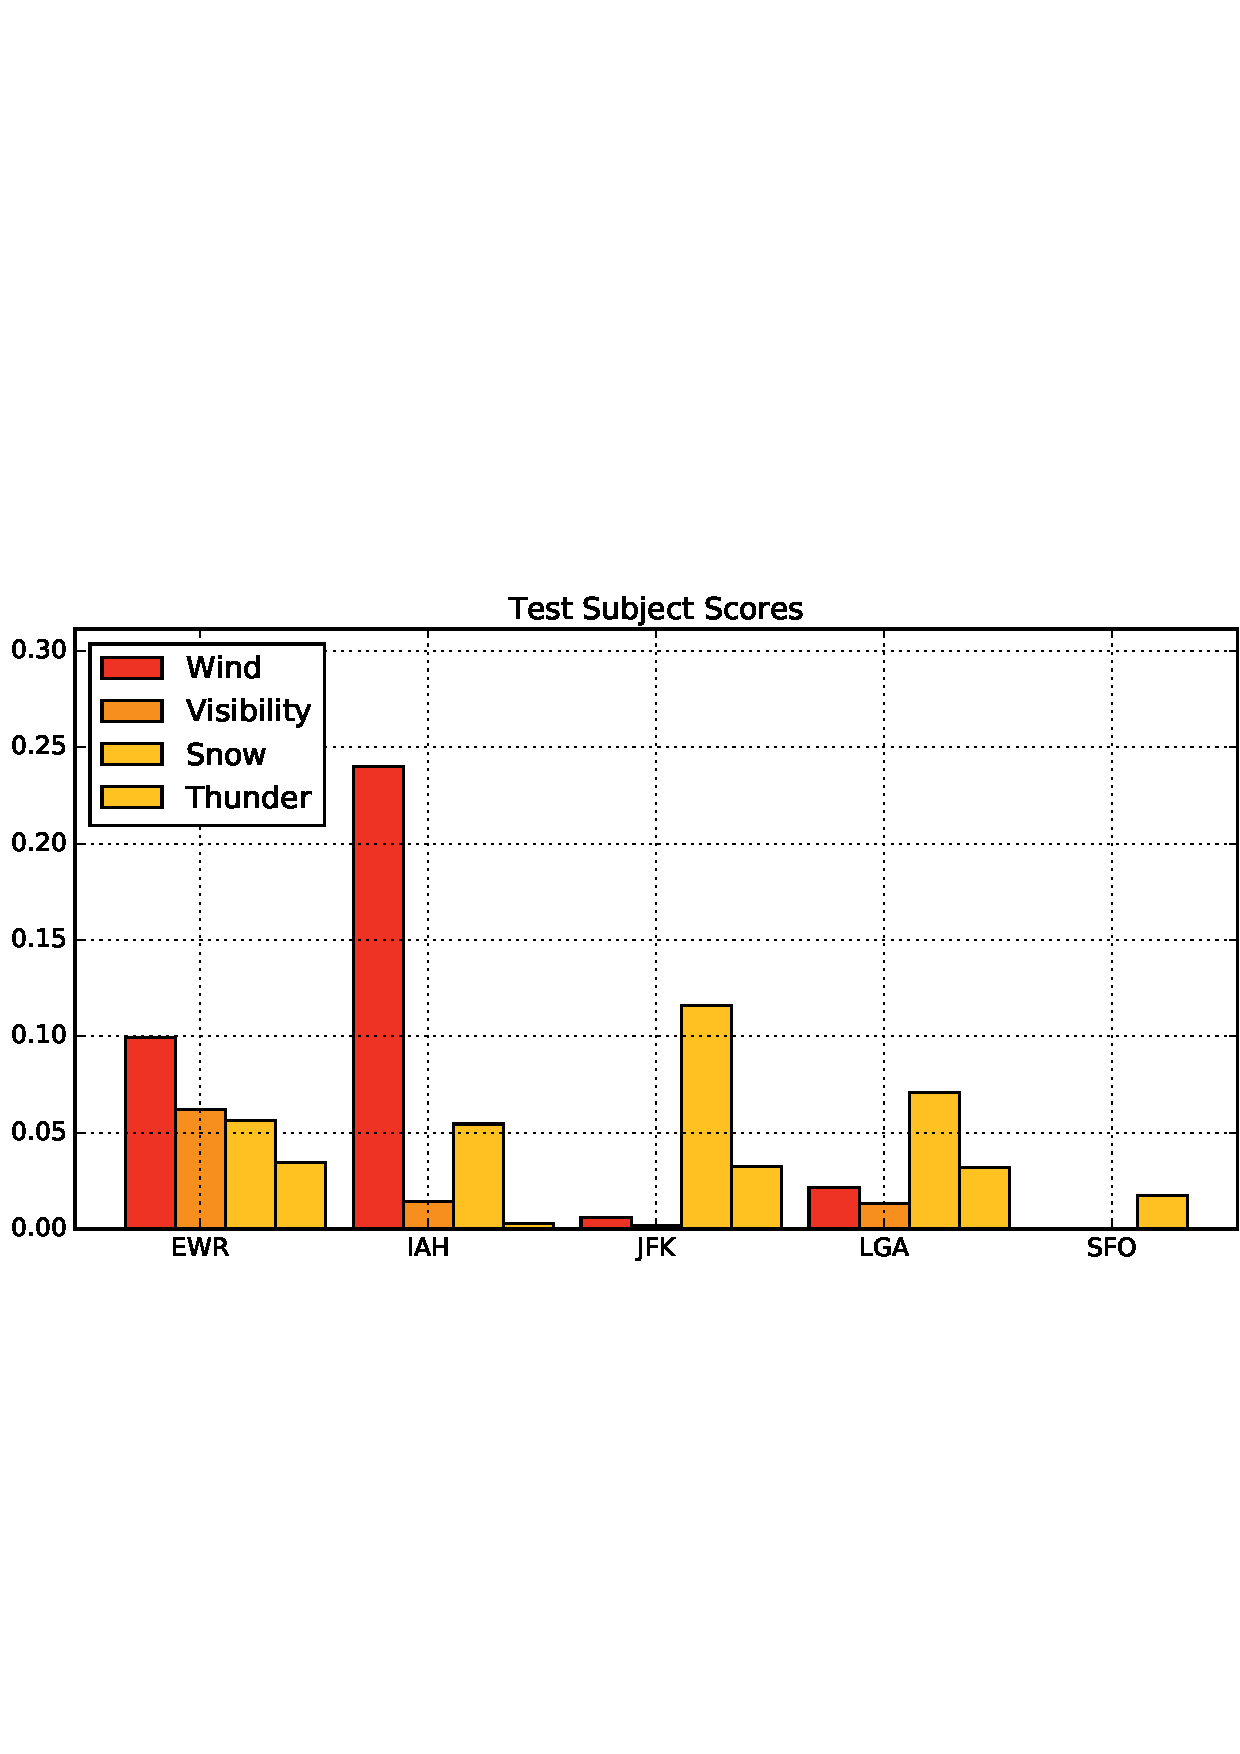
\includegraphics[height=4.3cm,width=1.2\linewidth]{Figures/ATT.png}
\caption{\scriptsize Effect of Weather on Flight Delay}
\label{sfig:testaa}
\end{subfigure}\hfill
\begin{subfigure}{0.33\linewidth}
\centering
\hspace*{-.23cm} 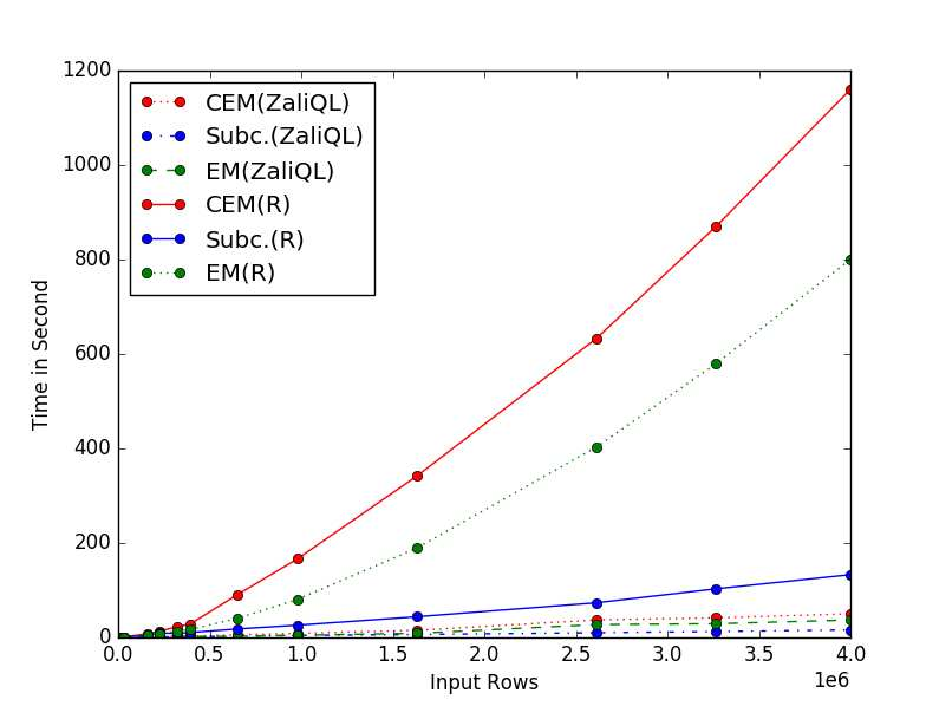
\includegraphics[height=4.3cm,width=1.1\linewidth]{Figures/exact.png}
\caption{\scriptsize Scalability Comparison (Subclassification)}
\label{sfig:testbb}
\end{subfigure}\hfill
\begin{subfigure}{0.33\linewidth}
\centering
\hspace{-.3cm}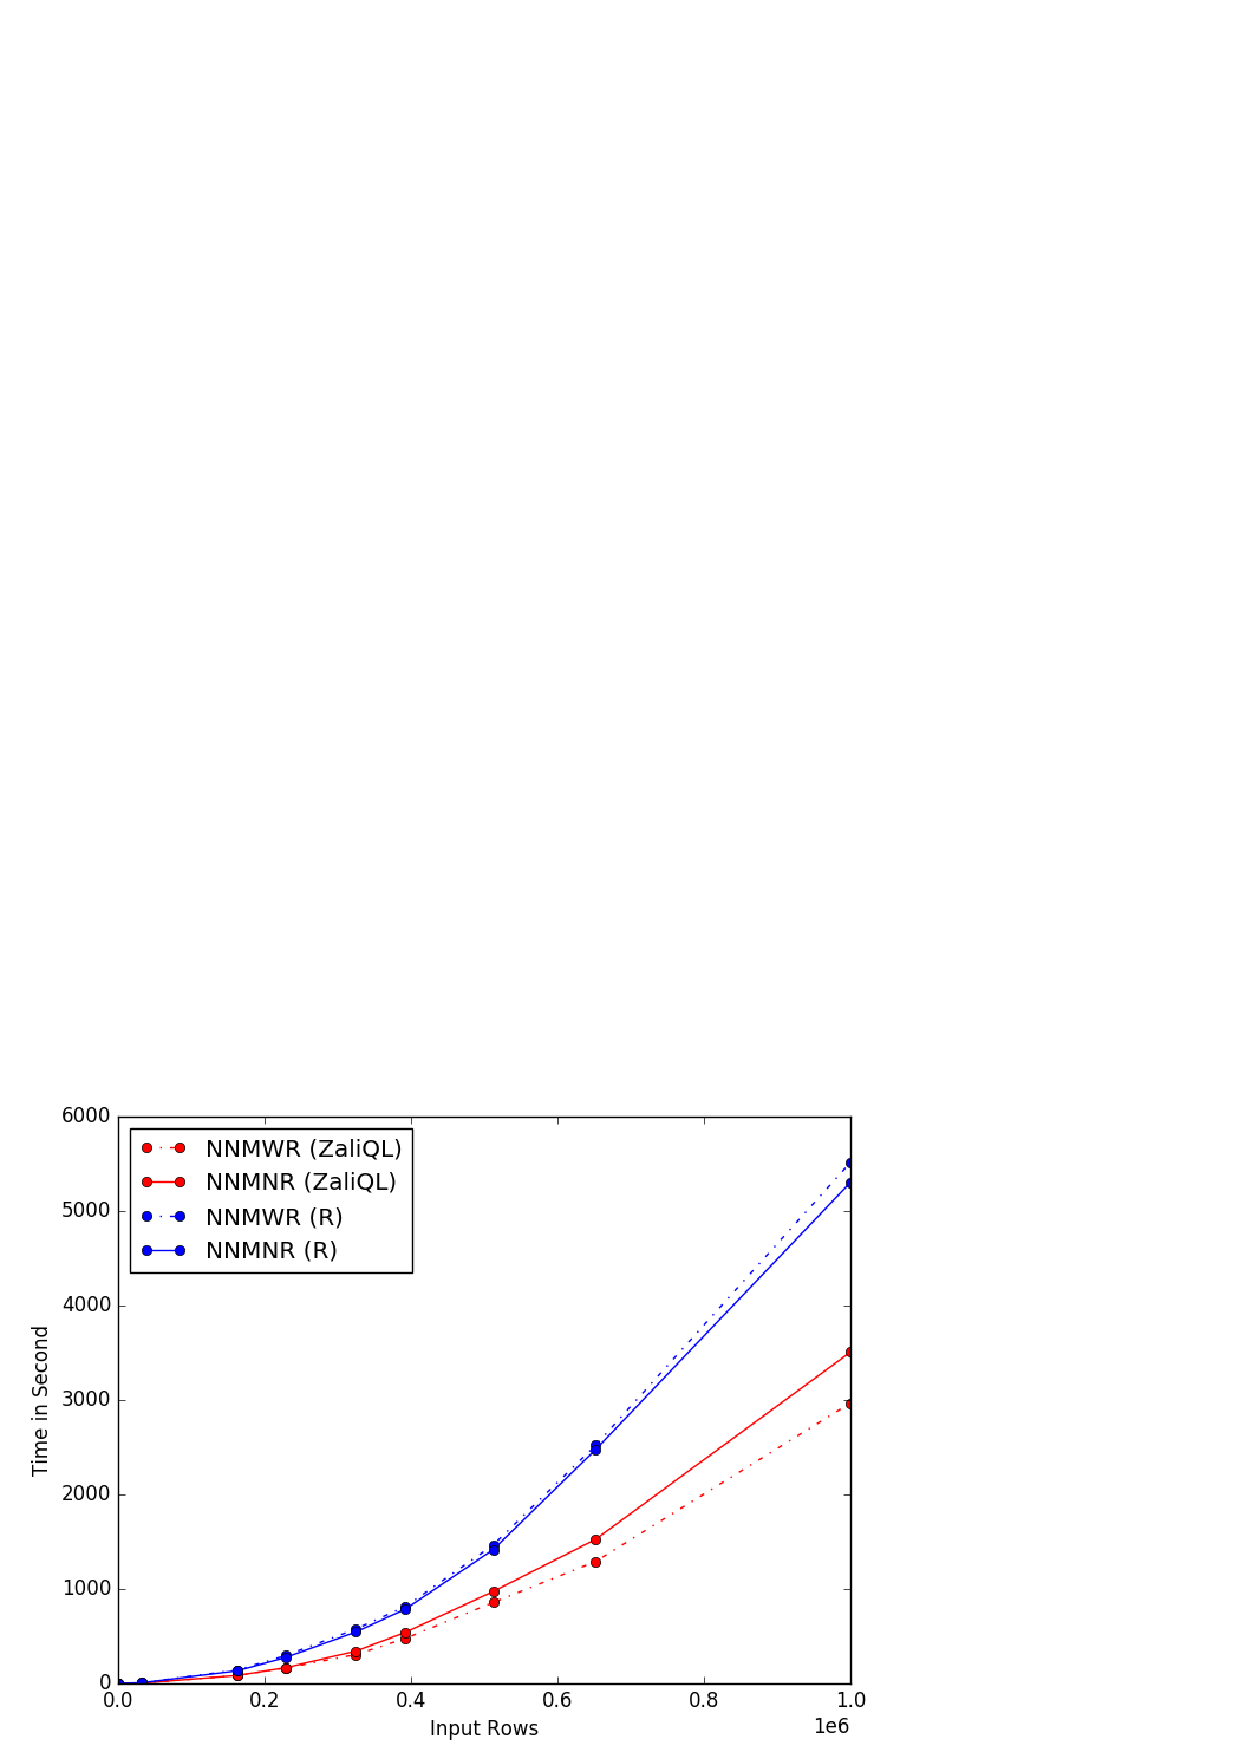
\includegraphics[height=4.3cm,width=1.1\linewidth]{Figures/NNM.png}
\caption{\scriptsize Scalability Comparison (Matching)}
\label{fig:push}
\end{subfigure}\hfill
\caption{{ (Results from preliminary work)~~ Performance and Scalability Evaluation of \GSQL}: we explored: nearest neighbor matching
 with and without replacement (NNMNR and NNMNR, respectively); subclassification bases on exact distance (EM), coarsen exact distance (CEM) and propensity score (Subc.)}
\label{fig:perfresults}
		\vspace{-0.3cm}
\end{figure*}
}

\ignore{
\subsection{Analyzing performance}

 We
explored four candidate causes for flight departure delays and
cancellations: Thunder, WindSpeed, LowVisibility, and Snow.  For
example ``what is the causal effect of {\em Thunder} (a Boolean
attribute in the weather data) on flight departure delay and
cancellation''.  As an illustration, Fig.~\ref{fig:perfresults}(a)
shows the results for delays at various airports: Thunder has the
largest causal effect at IAH (Houston, TX) and EWR
(Newark, NJ), while snow has the largest causal effect at JFK and LGA
(both in New York, NY); we note that these findings are consistent
with the finding. More interestingly we investigated the performance of our
subclassification and matching techniques expressed in SQL with state
of the art tools in R namely, MatchIt \cite{ho1737matchit}
and CEM \cite{iacus2009cem}. The performance for subclassification improves
by two orders of magnitude (Fig.~\ref{fig:perfresults}(b)) and for matching by a
factor of 2 (Fig.~\ref{fig:perfresults}(c)).
}





\section{Conclusions}
In this demonstration, we introduce \GSQL: a tool for
performing causal inference
on large relational data within a DBMS. \GSQL\ makes the first step towards truly scalable causal inference by modeling it as a data management problem. \GSQL\ implements a wide range of methods for causal inference developed in statistics with existing techniques
in data management. This provides scalable evaluation of several causal hypotheses
on relational data. \ignore{\GSQL\ is optimized for PostgreSQL and also includes a visual interface to wrap around the framework.}

\section{ACKNOWLEDGEMENTS}
This work is supported in part by the National Science Foundation through NSF grants IIS-1614738 and
University of Washington's CSE Postdoc Research Award.

% The following two commands are all you need in the
% initial runs of your .tex file to
% produce the bibliography for the citations in your paper.
\bibliographystyle{abbrv}
\bibliography{vldb_sample}  % vldb_sample.bib is the name of the Bibliography in this case
% You must have a proper ".bib" file
%  and remember to run:
% latex bibtex latex latex
% to resolve all references


\end{document}
